\section{Methodology}
\label{sec:methodology}

\begin{figure}[t]
    \centering
    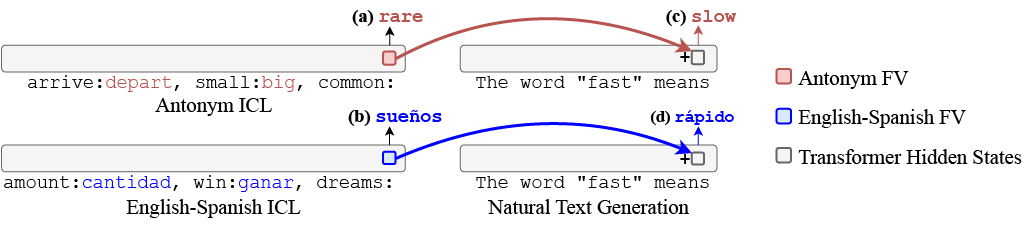
\includegraphics[width=0.95\linewidth]{figures/method_overview.png}
    \caption{Overview of the \fv mechanism for summarization. We extract hidden state activations at the final prompt token during few-shot prompts across style-specific datasets (\cnndm and \xsum) to isolate stylistic constraints.}
    \label{fig:method_overview}
\end{figure}

Our methodology aims to generalize the \fvabbr framework to complex summarization tasks and decode stylistic constraints (\extractive vs. \abstractive) from the resulting vectors.

\subsection{Datasets}
We selected two summarization datasets with opposing default stylistic constraints:
\begin{itemize}[leftmargin=*,itemsep=0pt,topsep=0pt]
    \item \cnndm (\extractive bias): A large-scale dataset of news articles with multi-sentence, \extractive summaries typically formatted as bullet points~\cite{hermann2015teaching}.
    \item \xsum (\abstractive bias): A dataset of news articles where each summary is a single, highly compressed, and \abstractive rephrasing of the original text~\cite{narayan2018dont}.
\end{itemize}
These datasets provide a natural contrast between two major summarization paradigms, allowing us to isolate the representation of these stylistic constraints.

\subsection{Activation Extraction Protocol}
We used activation extraction via the \textsc{baukit} library~\cite{bau2019visualizing} to capture the hidden states of \gpttwo (1.5B parameters) during few-shot summarization. Our goal was to obtain a holistic snapshot of the ``task context'' for each summarization style.

For both \cnndm and \xsum, we formatted articles into 2-shot prompts. We then captured the mean hidden states (\newterm{Layer \fvsabbr}) across 10 trials at the final prompt token (the token immediately preceding the summary generation, \ie, the final token of the ``Summary:'' structure). This process was repeated for each of the 48 layers of the model.

\subsection{Intervention Strategy}
To evaluate the causal efficacy of the extracted vectors and their ability to steer generation, we performed a zero-shot intervention. We injected a \newterm{difference vector} into the model during generation:
\begin{equation}
    \vh_{\ell} \gets \vh_{\ell} + \alpha (\vv_{\textsc{CNN}, \ell} - \vv_{\textsc{XSum}, \ell})
\end{equation}
where $\vh_{\ell}$ is the model's hidden state at layer $\ell$, $\vv_{\textsc{CNN}, \ell}$ and $\vv_{\textsc{XSum}, \ell}$ are the extracted layer-wise vectors, and $\alpha$ is a scaling factor. We initially targeted layer 24 (the middle layer) for this intervention to assess whether the stylistic constraints are already disentangled and manipulatable at this stage.

\subsection{Evaluation Metrics}
We evaluated the similarity between extracted vectors using cosine similarity across all layers. For generation performance, we used the standard \rouge metric~\cite{lin2004rouge}, reporting \rougeone, \rougetwo, and \rougel scores to compare baseline and intervened generations.
